% !TEX root = ../Yan Hao-Dissertation.tex

\chapter{Introduction} \label{chapter1:Introduction}

\section{About Fiscal Federalism}
The field of fiscal federalism studies how to divide responsibilities (including finances) among federal, state, and local governments to improve economic efficiency and achieve various public policy objectives.Determining the optimal division of responsibilities and funding is difficult because of varying subjective views about what the role of government should be. As a result, fiscal federalism research generally renders no judgment on the proper level of total government intervention or what types of services governments should provide. The research focuses instead on how responsibilities are assigned across multiple layers of government once policymakers have decided to implement a given policy, and what trade-offs may be involved in administering it. To be more specific, Central and local governments have their own way to generate revenue and supply public goods and services separately. Besides, central government compensate the low income subnational government by doing transfer payments,which is so called intergovernmental transfer, so local governments especially the low-income local government still got the ability to supply the necessary public goods and services. To summarize, central and local governments got the ability to collect the revenue so to supply the necessary public goods and services with the consideration to achieve the political intention. Depend on the general fiscal federalism setting, I'll give an overall view of the fiscal federalism structure in the rest of this chapter. Three key points are vital for the understanding: the revenue source for different levels of government, the public service responsibilities,and the financial connection between central and subnational governments, as is shown in Figure \ref*{Figure 1.1}

\begin{figure}[htb]
    \centering
    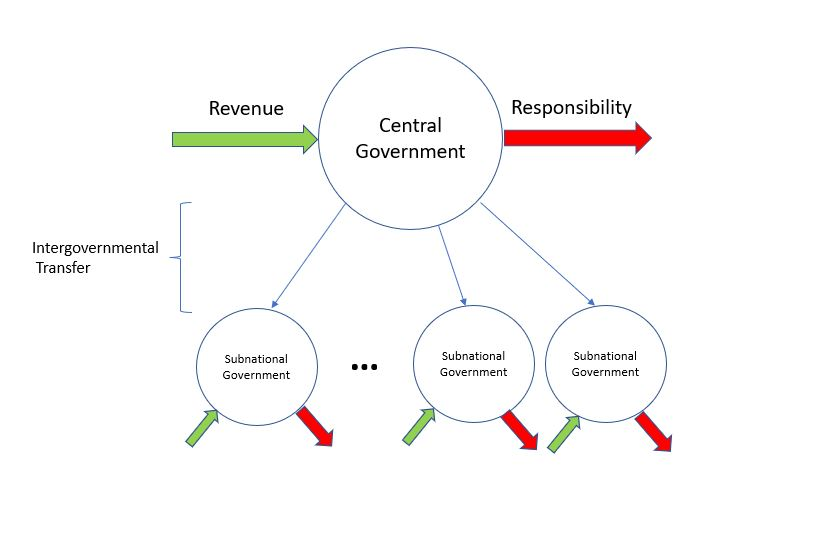
\includegraphics[scale=0.7]{Chapter-1/Figures/fiscal federalism.JPG}
    \caption[Fiscal Federalism Structure]{Fiscal Federalism Structure
        \texttt{} }
    \label{Figure 1.1}
\end{figure}

For the following part of this chapter, I'll give a basic introduction about the fiscal federalism structure in USA, to be more specific, I'll describe the revenue and responsibilities of different levels of governments, and the intergovernmental transfer between different levels of governments.



\subsection{Fiscal Federalism Structure in America}
\subsubsection{Revenue and Responsibilities of different levels governments}
The United States constitution stipulated that states keep the remaining rights, which means except for the clear defined rights that federal government have, states government keep the undefined rights. Besides, the constitution set no instruction about the responsibilities between state and local governments. This feature combined with the fact that America is a huge country with rich diversity lead to an interesting administrative fact: the responsibilities of state governments in each states are not identical. Within each states, the local governments form up their responsibilities based on the actual needs, thus the local governments are not identical neither. Thus the follow introduction are not describing the administrative reality precisely, but are introducing the general structure.

Under current fiscal federalism system in America, federal, state and local governments rely on different source of income, have different function in supplying the public good and federal government reimburse the state and local government through intergovernmental transfer. On revenue side, from the breakdown of the source of revenue of fiscal year 2019, 50\% of the federal revenue comes from the individual income tax, 7\% from corporate income tax, 36\% is social insurance or payroll tax. On the other hand, on state and local level, intergovernmental transfer accounts for more than 30 percent on average, followed by sales taxes and property tax.
%%%%%%%%%
\begin{figure}[H]
    \centering  %居中
    \subfigure[Source of Federal General Revenue]{   %第一张子图
        \begin{minipage}{7cm}
            \centering    %子图居中
            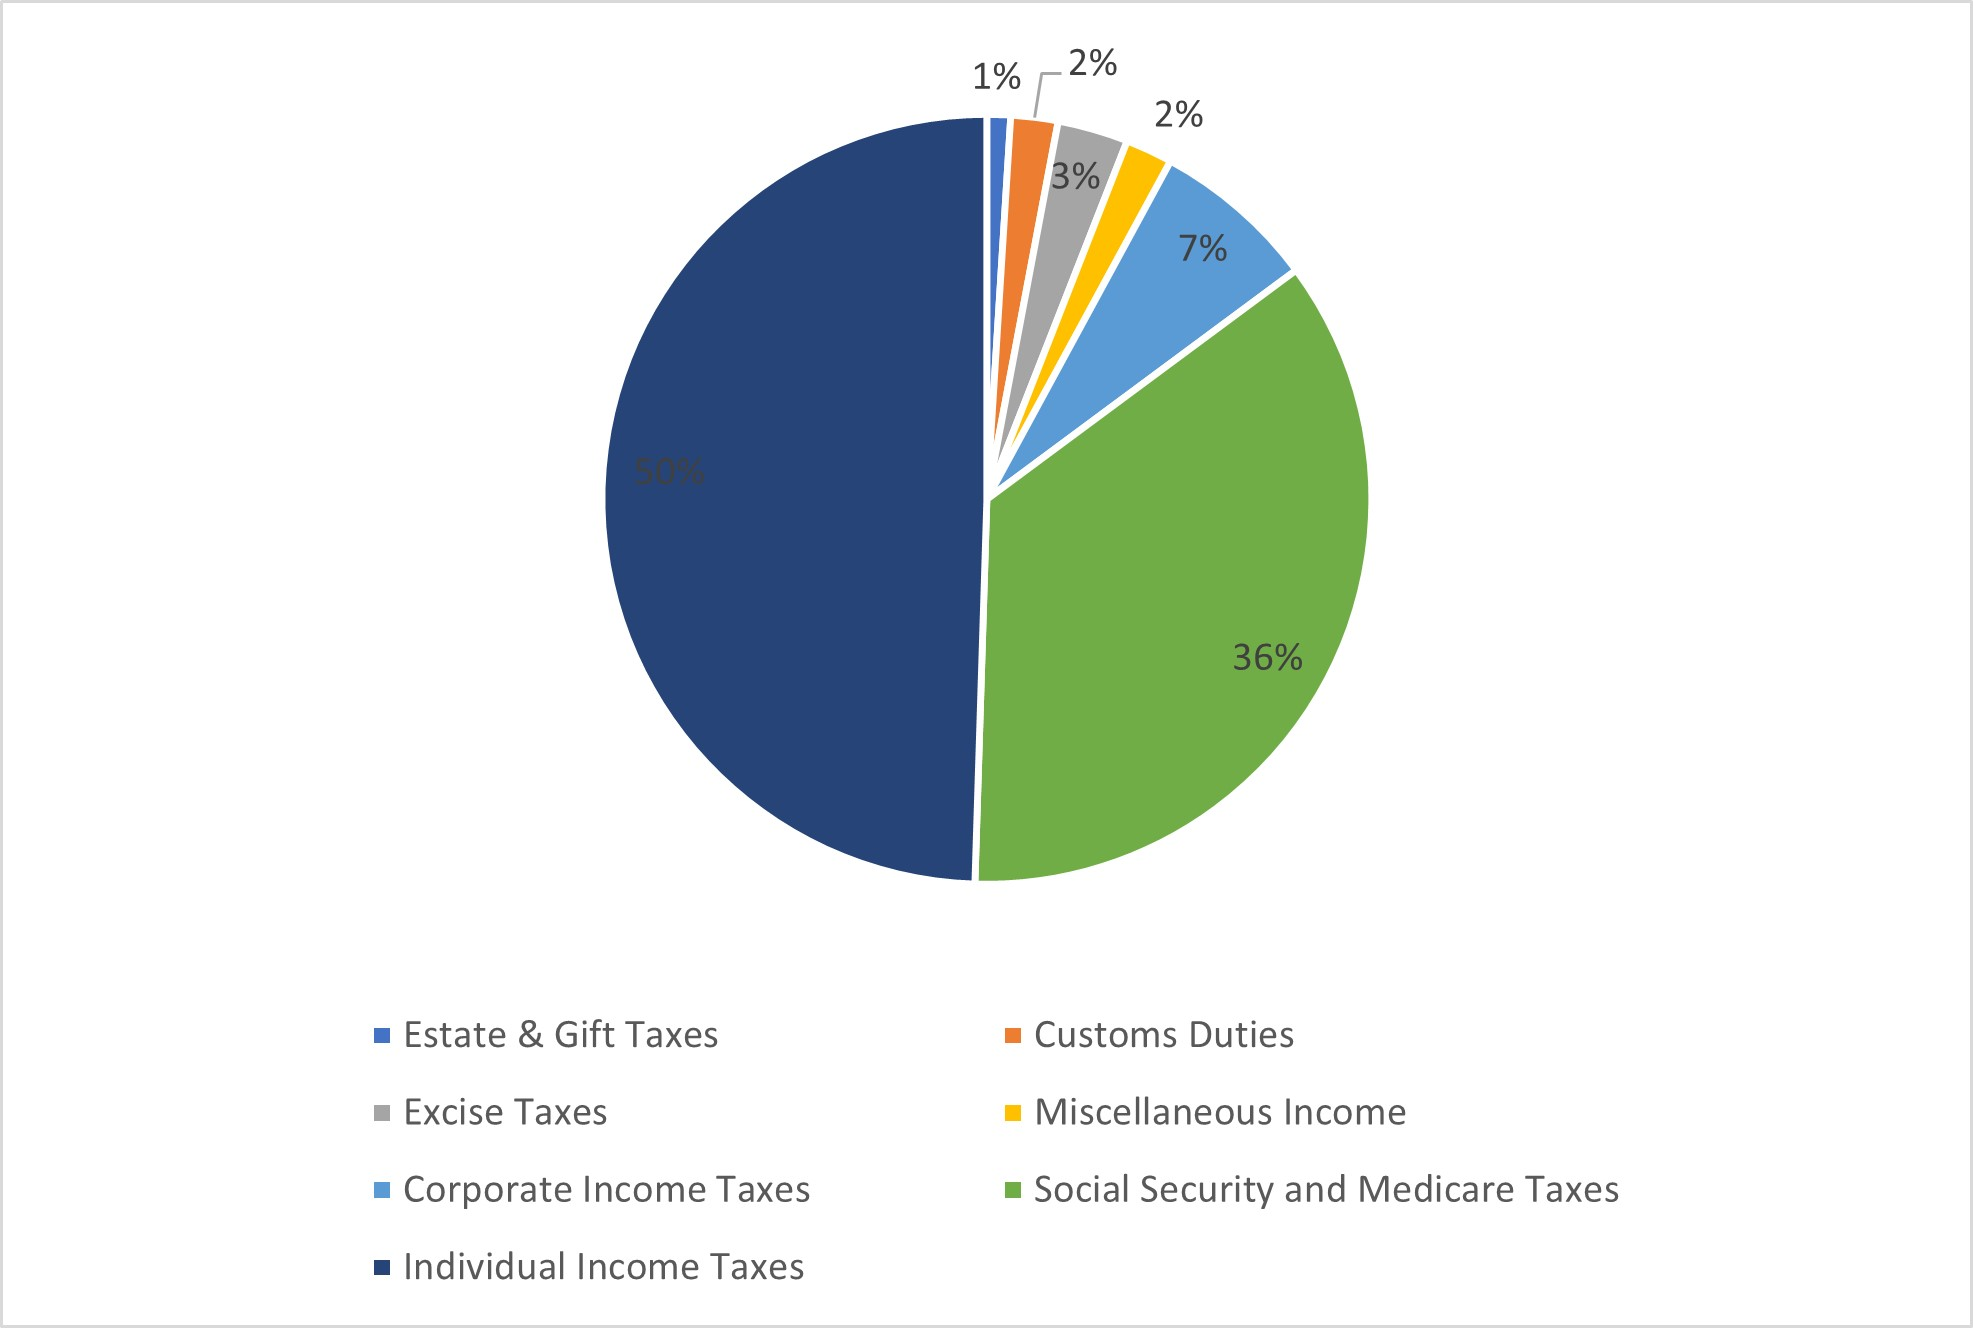
\includegraphics[scale=0.37]{Chapter-1/Figures/source of federal general revenue.jpg}  %以pic.jpg的0.5倍大小输出
        \end{minipage}
    }
    \subfigure[Source of State General Revenue]{ %第二张子图
        \begin{minipage}{7cm}
            \centering    %子图居中
            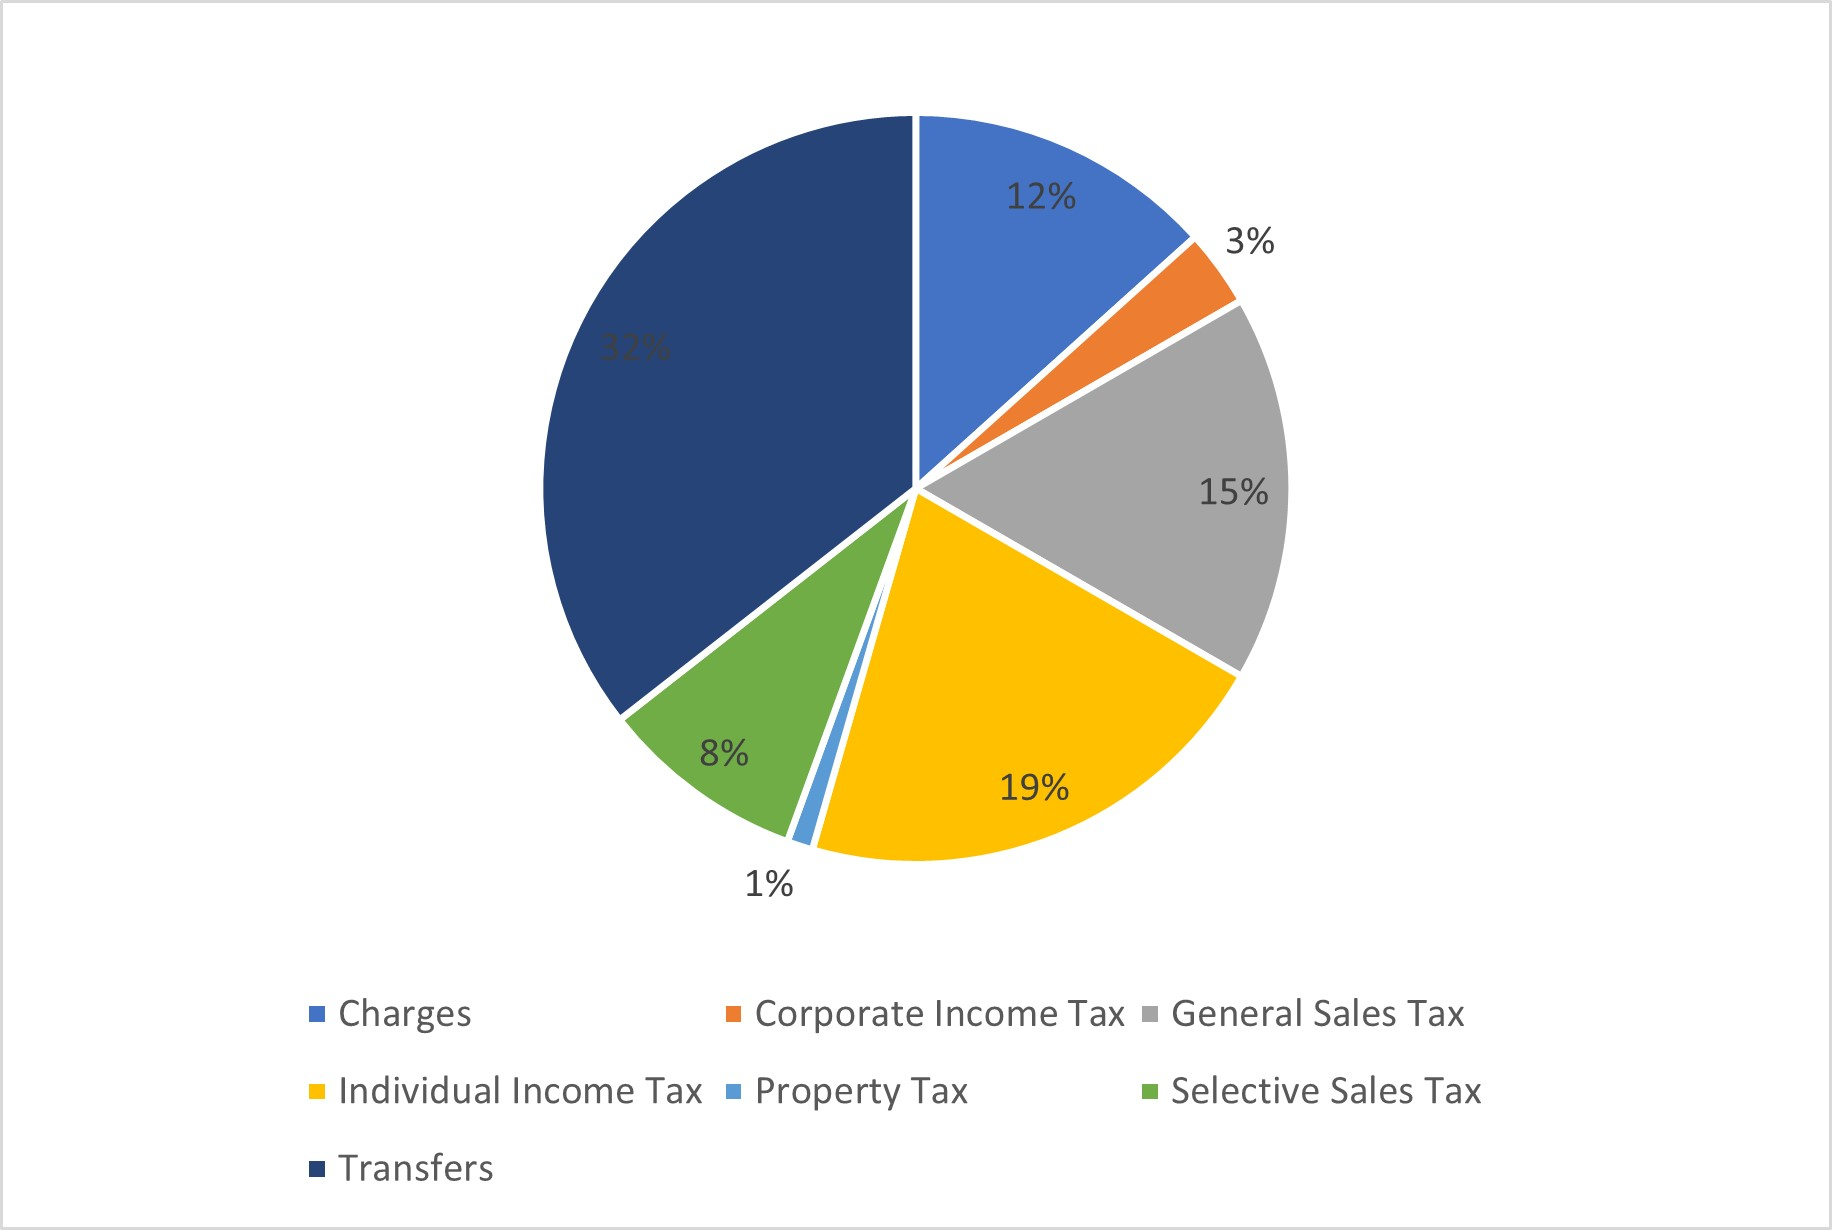
\includegraphics[scale=0.4]{Chapter-1/Figures/source of state general revenue.jpg}%以pic.jpg的0.5倍大小输出
        \end{minipage}
    }
    \subfigure[Source of Local General Revenue]{ %第三张子图
        \begin{minipage}{7cm}
            \centering    %子图居中
            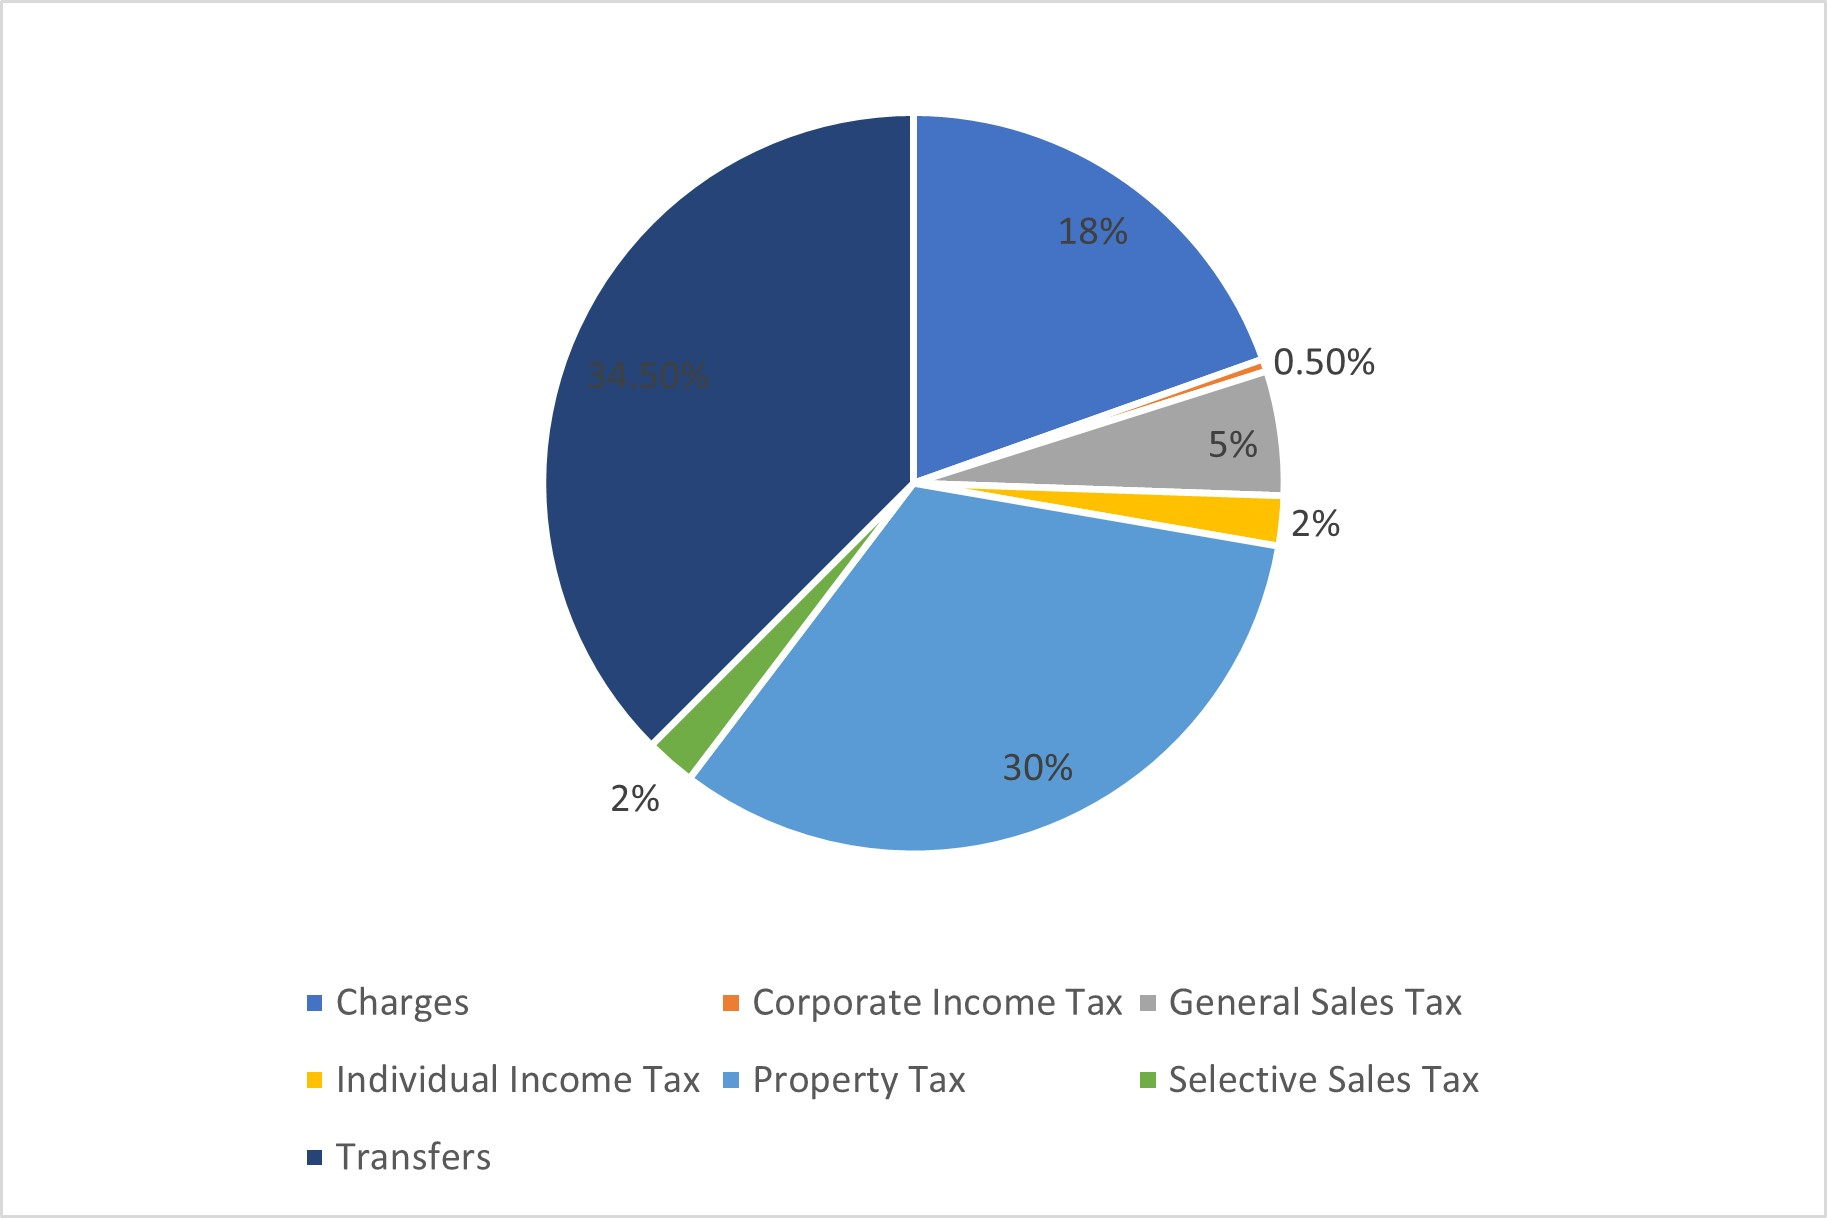
\includegraphics[scale=0.5]{Chapter-1/Figures/sources of local general revenue.jpg}%以pic.jpg的0.5倍大小输出
        \end{minipage}
    }
    \caption[Source of Revenue for Multiple Level of Governments in 2019]{Source of Revenue for Multiple Level of Governments.Data Source:The Department of the Treasury and the Bureau of the Fiscal Service }    %大图名称
    \label{Figure 1.2}    %图片引用标记
\end{figure}
%%%%%%%%%%%%%%%%%%%%%%%%%%    


%%%
%\begin{figure}[htb]
%    \centering
%    \includegraphics[scale=1]{Chapter-1/Figures/Revenue breakdown of United States}
%    \caption[Revenue breakdown of the different levels of governments in 2019.]{Revenue breakdown of the different levels of governments in 2019.
%    \texttt{Source: U.S. Census of Bureau} }
%    \label{Ch1-figure: Revenue breakdown of United States}
%\end{figure}
%%%

On the expenditure side, federal, state and local government functions differently in supplying public goods and services. Filtered out the public-goods-unrelated expenditure such as interest from debt, federal government is paying for income security, social security, health, national defense, highways and infrastructure, medic care, social services such as education, training and employment. Similarly, if filtered out the expenditure which are unrelated to the public goods and services in state and local governments, the left parts include public welfare, elementary and secondary education, higher education, health and hospitals, highways and roads, police, courts, housing and community development.
%%%
%%%%%%%%%%%%%%%%%%%%%%%%%%%%%%%%%%
\begin{figure}[H]
    \centering  %居中
    \subfigure[Federal Expenditure]{   %first subfigure
        \begin{minipage}{7cm}
            \centering    %子图居中
            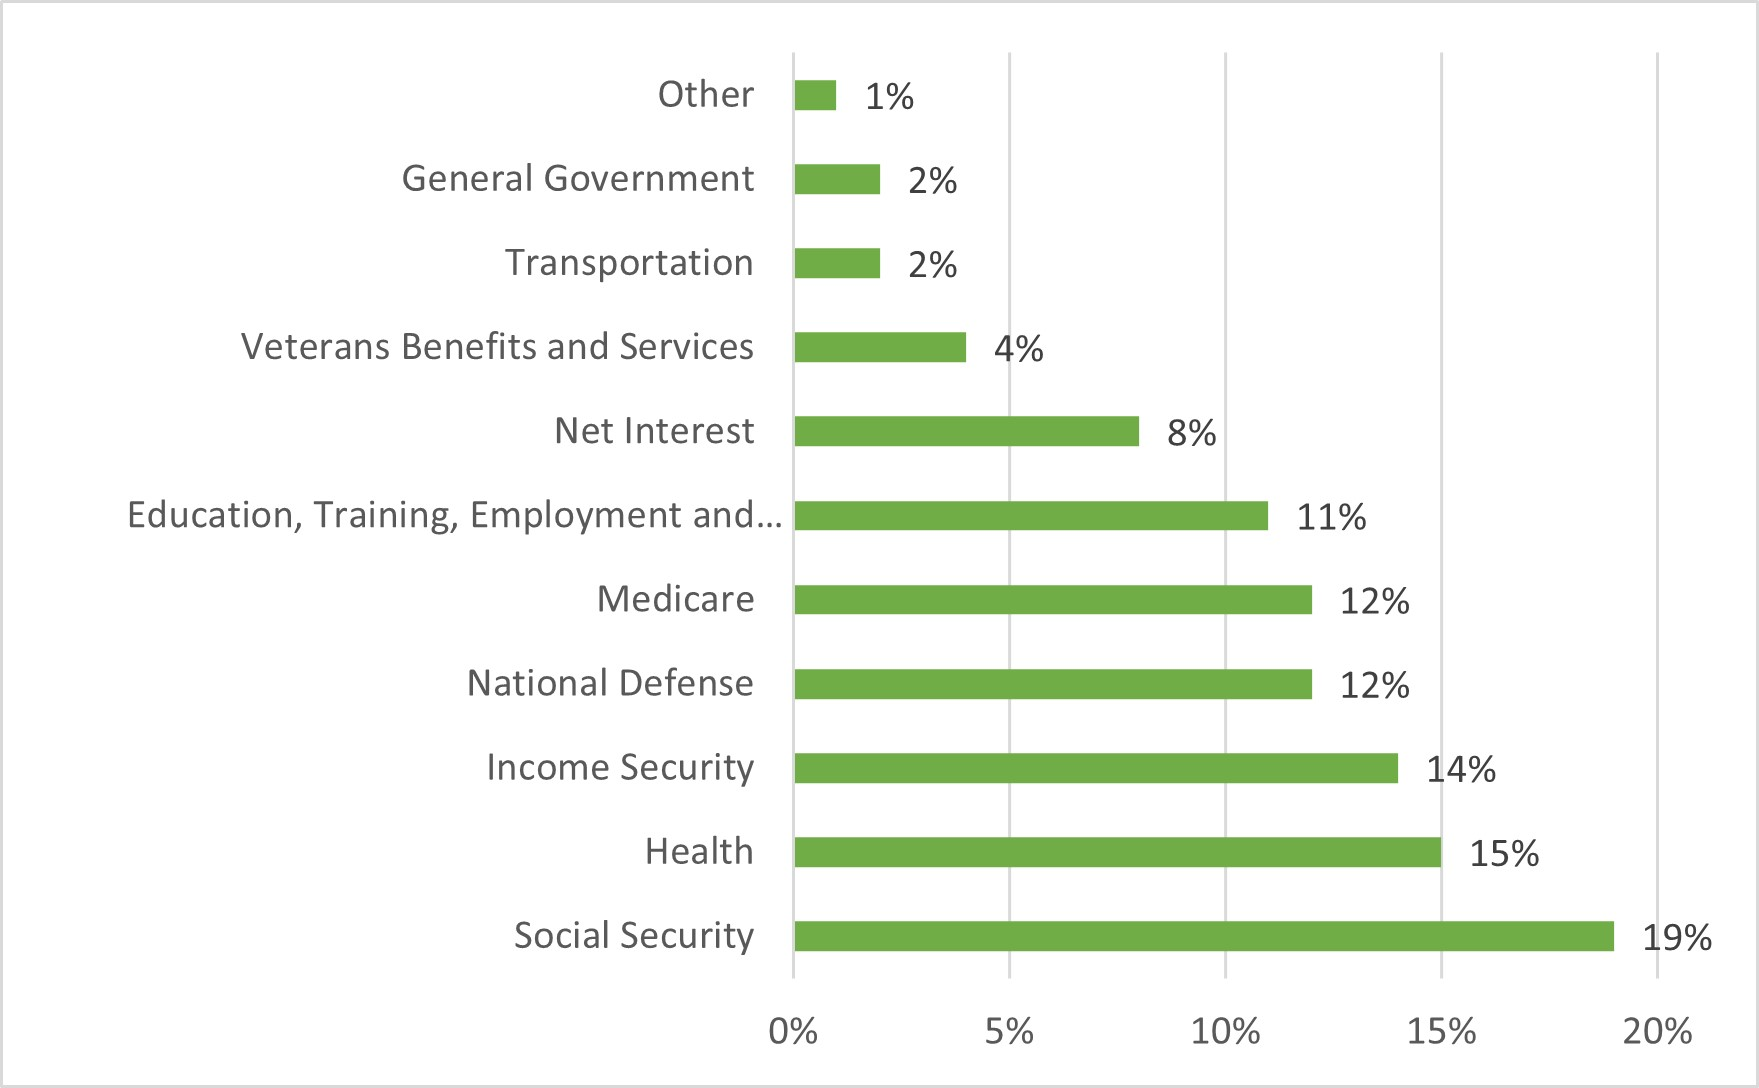
\includegraphics[scale=0.52]{Chapter-1/Figures/federal expenditure.JPG}  %以pic.jpg的0.5倍大小输出
        \end{minipage}
    }
    \subfigure[State and Local Expenditure]{ %second subfigure
        \begin{minipage}{7cm}
            \centering    %子图居中
            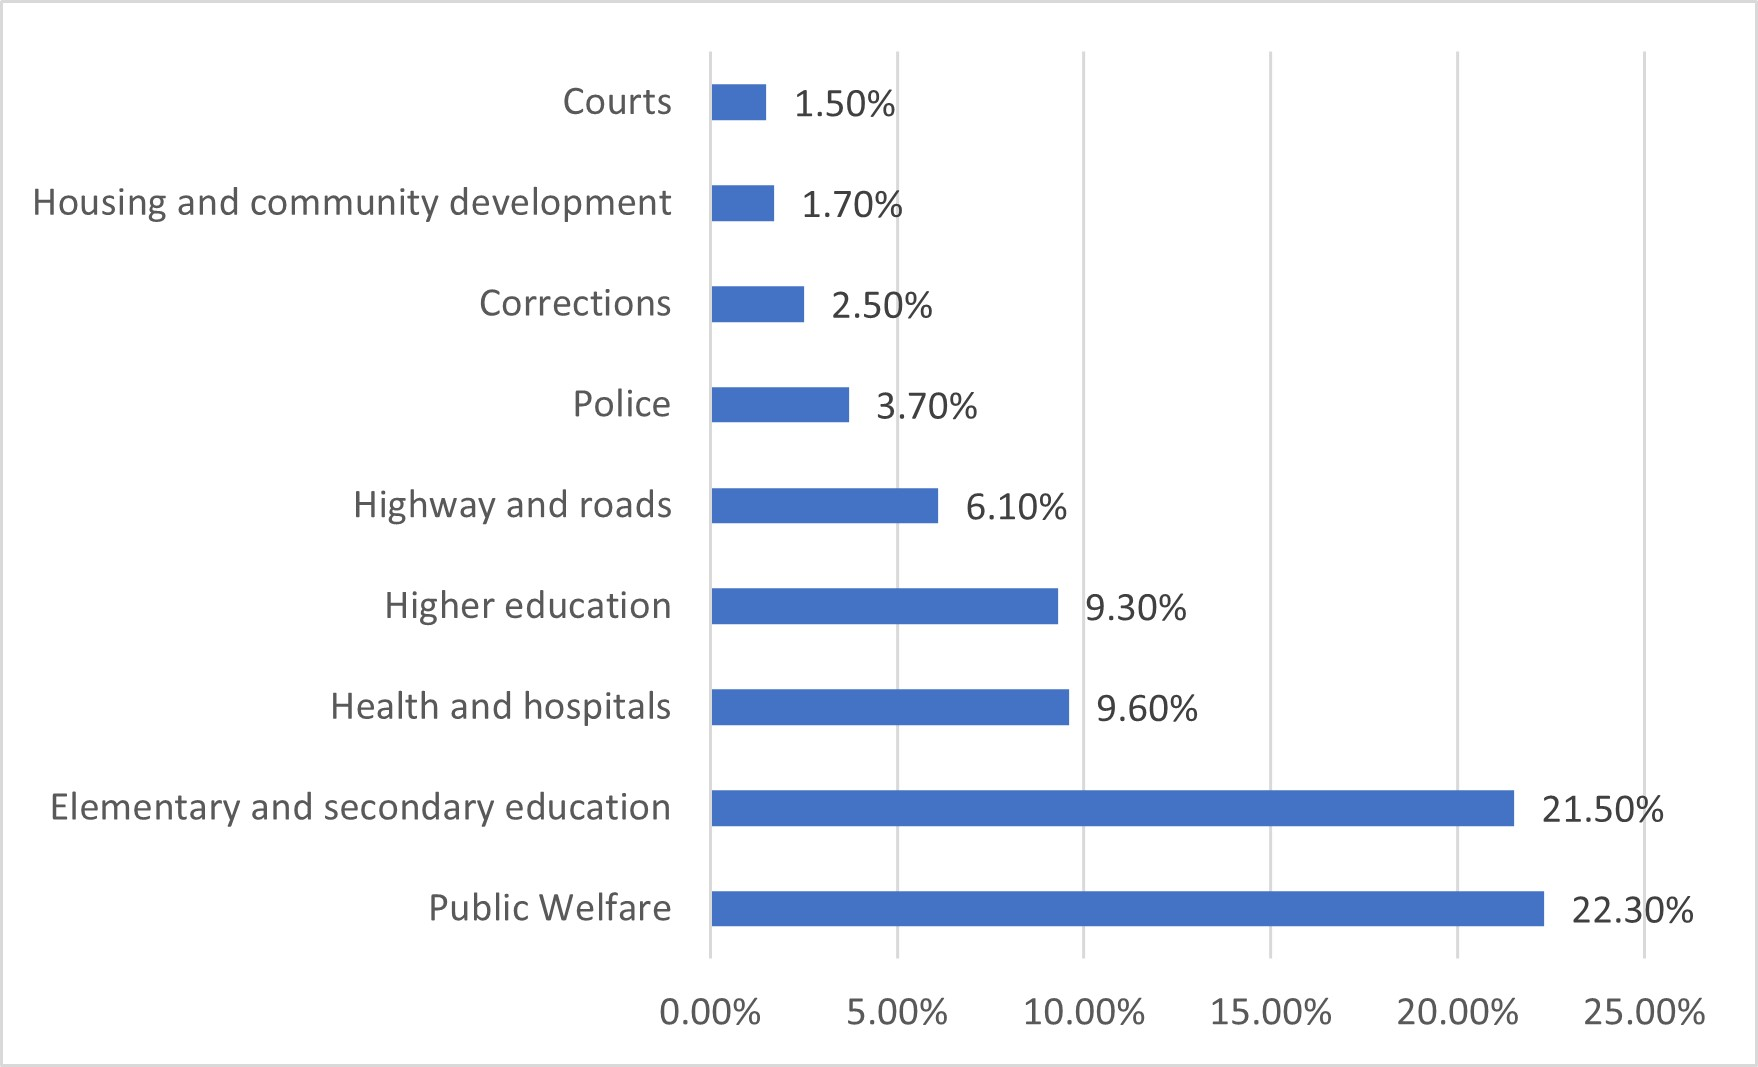
\includegraphics[scale=0.52]{Chapter-1/Figures/state and local expenditure.JPG}%以pic.jpg的0.5倍大小输出
        \end{minipage}
    }

    \caption[Source of Revenue for Multiple Level of Governments in 2019]{Source of Revenue for Multiple Level of Governments.Data Source:The Department of the Treasury and the Bureau of the Fiscal Service }    %caption for whole figure
    \label{Figure 1.3}
\end{figure}

Though The revenue and expenditure structure of federal, state and local government are relatively stable. Figure\ref*{Figure 1.3} shows a cross-sectional data of 2019. A time series fluctuation is presented in Figure\ref*{Figure A.1} attached in Appendix A. Information in Figure\ref*{Figure A.1} shows that it's not a big deal to capture the revenue structure by just breakdown the data in one year.


Federal, state and local government has their unique function in supplying public goods, for example, the federal government is supplying national defense exclusively, while state and local government is the sole supplier in police, courts, housing and community development. Meanwhile, some of the areas are overlapped by both layers of governments, such as public welfare, education, health, highway and infrastructure construction.

\begin{figure}[H]
    \centering
    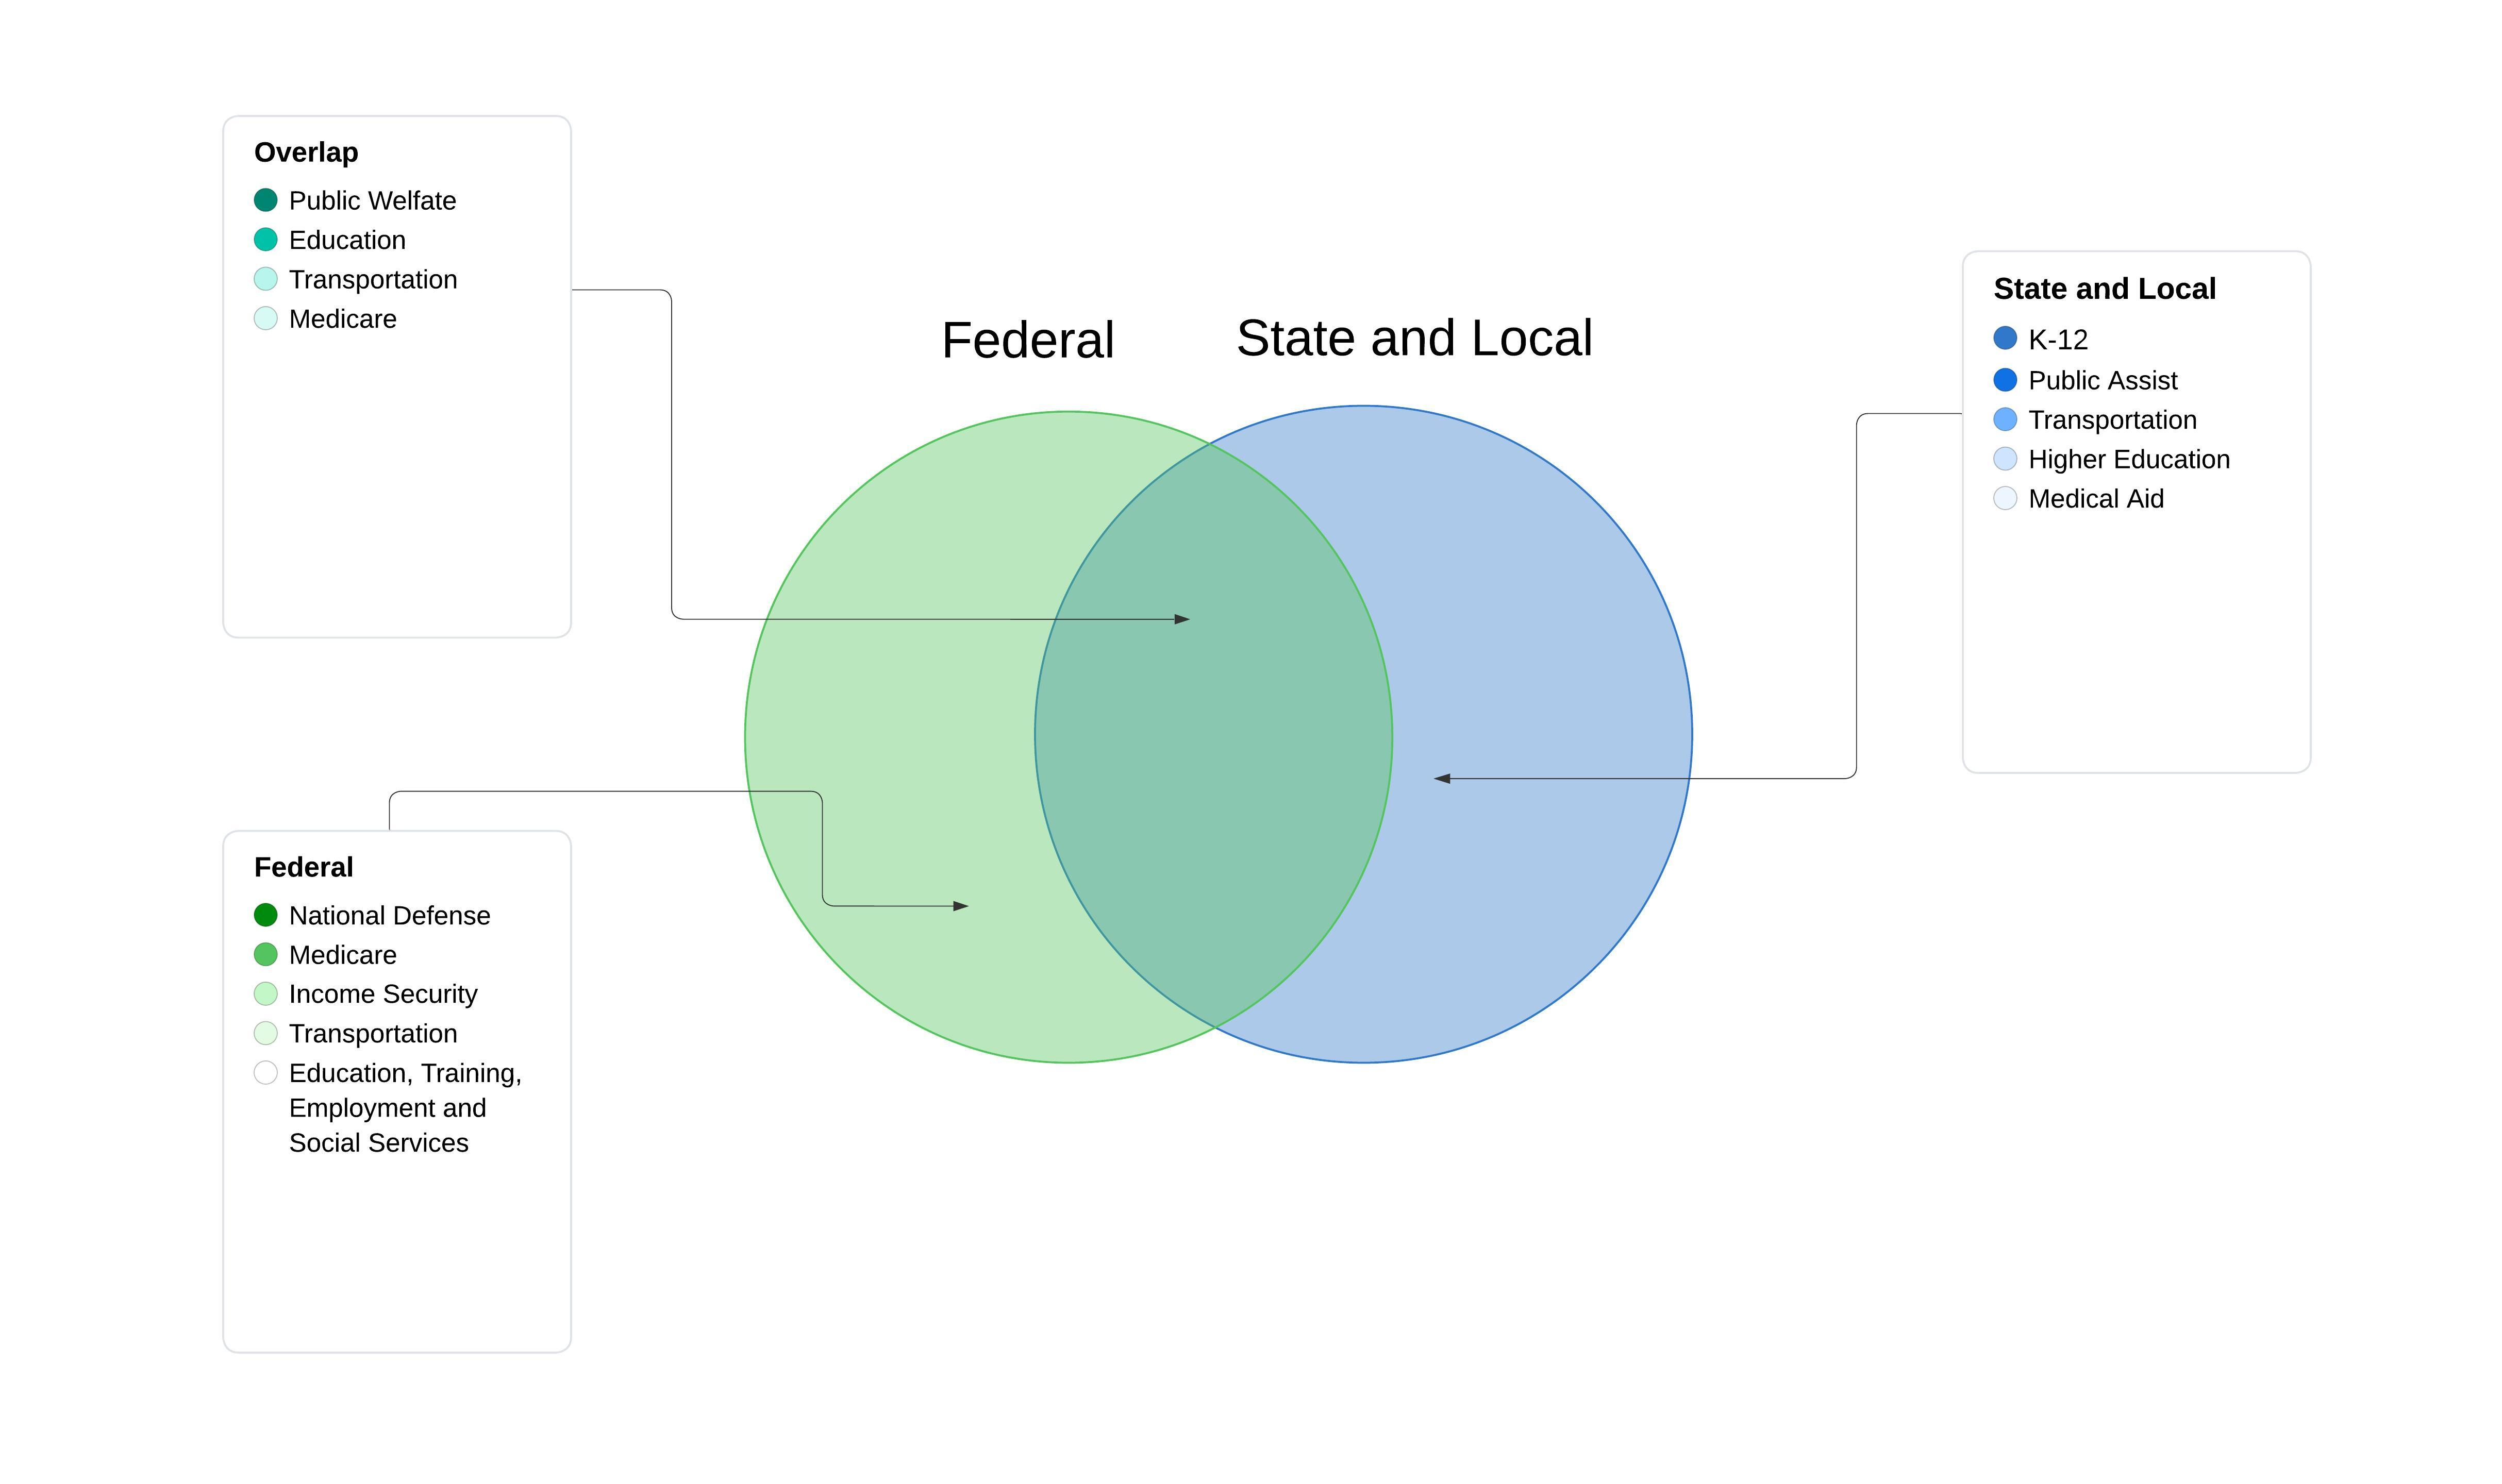
\includegraphics[scale=0.4]{Chapter-1/Figures/Venn graph on public goods.jpeg}
    \caption[Venn graph on public goods and services supplying]{Venn graph on public goods and services supplying by federal, states and local government
        \texttt{} }
    \label{Figure 1.4}
\end{figure}

\subsubsection{Intergovernmental Transfer in America}
In the US fiscal federal system, the Federal government imposes significant influence on state and local fiscal decision making through various grants-in-aids programs (GIA) or intergovernmental transfer(IGT). Annually, these programs amounts to nearly \$700 billion, or close to 20 percent of overall federal revenues \cite{dilger2015federal}. Grounded in fiscal federalism, these programs, are guided by the idea that the allocation of publicly funded goods and services should be the responsibility of state and local governments, due to their closer proximity to the constituents. The sought for advantages of such division include: reduced costs associated with planning and administration, the ability to account for spatial differences, and increased opportunities for citizens to influence political decision-making \cite{musgrave1997devolution}. IGT from federal government help to narrow the gap between revenue and expenditure of state and local government, encourage the supply of specific public goods and promote the horizontal equity among states

%%%%%%%%%%
Generally, grants-in-aids programs in the US federal fiscal system, can be categorized across two dimensions including the level of restrictions that are attached to the awards, and the administrative procedures that govern the award process. In terms of restrictions, GIAs can be organized into categorical grants, block grants and general revenue sharing grants. Categorical grants include formula categorical grants, open-ended reimbursement categorical grants and project categorical grants.Project categorical grants are awarded with relatively strict set of activities that are attached to a specific purpose. Block grants are awarded to fund specific programs, but carry relatively few restrictions. The main difference is that block grants do not attach a specific purpose to how recipients spend the award. General revenue sharing grants carries the least amount of restrictions. In brief, these awards can be spent for any purpose, as long as it is not prohibited by federal or state law.  According to the Congressional Research Service report \cite{dilger2015federal}, there are about 600 grant-in-aid programs, and categorical grants account for about 95 percent of the programs and more than 80 percent of total grant outlays.

% Table generated by Excel2LaTeX from sheet 'Sheet1'
\begin{table}[H]
    \centering
    \caption{Divide Grants by level of Restriction Attached}
    \begin{tabular}{ccc}
        \toprule
        \multicolumn{3}{c}{Level of Restriction}                                   \\
        \midrule
        Low Restriction           & Medium Restriction & High Restriction          \\
        \midrule
        Formula Categorical Grant & Block Grant        & Project Categorical Grant \\
        Open-ended Reimbursement  &                    &                           \\
        General Revenue Sharing   &                    &                           \\
        \bottomrule
    \end{tabular}%
    \label{Table 1.1}%
\end{table}%



In terms of the administrative procedures that govern the awards, the grants can be categorized into three categories including projects grants or competitive grants, formula grants/formula-project grants, and Reimbursement grants. For competitive grants, states should apply by submitting a request and get the grants through a competitive process. They are intended to improve the efficiency of funding allocation by encouraging grantees to seek funds for well-planned and exemplary projects. Formula grants are distributed to states through mathematical formulas decided by social characters within the jurisdiction. Typically the factors in the formula depends on the intention of the grants, and common factors may include population, poverty level, income per capita, unemployment rate, enrollment in public schools, etc. Finally, reimbursement grants awards state and local governments in the form of a reimbursement for a specific percentage of state and local spending on a program.The reimbursement amount does not carry a specific limit. Reimbursement grants could be divided into open and closed ended reimbursement grants. The matching mechanism in reimbursement grants is a very intriguing consideration in public economic literature when evaluating the distortion effect. For matching grants, federal governments will reimburse a specific ratio for each 1 dollar of state and local expenditure. Based on whether federal government set a cap on the matching grants, matching grants can be divided into open-ended matching grants and closed-ended grants.



% Table generated by Excel2LaTeX from sheet 'Sheet2'
\begin{table}[htbp]
    \centering
    \caption{Divide Grants by Form of Administrative Procedure}
    \begin{tabular}{clc}
        \toprule
        \multicolumn{3}{c}{Form of Administrative Procedure}                                                                                                     \\
        \midrule
        \multicolumn{1}{p{9.645em}}{ Submitting Request} & \multicolumn{1}{p{10.285em}}{               By Formula} & \multicolumn{1}{p{10.855em}}{Reimbursement} \\
        \midrule
        \multicolumn{1}{l}{Competitive Grants}           & Formula grants                                          & Project Categorical Grant                   \\
                                                         & Formula-project grants                                  &                                             \\
        \bottomrule
    \end{tabular}%
    \label{Table 1.2}%
\end{table}%




%\subsection{Fiscal Federalism Structure in China}

\subsection{Introduction of the Structure in the Following Chapters}
The goal of this paper is to systematically describe the fiscal federalism structure, explain some of the fiscal phenomenon in the administrative process on the theoretical level using some game theory tool and empirically test the theory I brought up, especially in America. I form the paper by asking and trying to answer a series of questions. The general questions in this research can be divided into theoretical questions and practical questions. Theoretical questions are asking what an ideal framework should be, and practical questions are asking what the actual situation is and I will try to explain the gap between the theoretical design and actual administrative reality. Besides, at least two layers of governments exists in fiscal federalism structure, so by asking theoretical questions and practical questions in two layers of government, I can generate a $2\times2$ table shown in Table \ref*{Table 1.3}.

% Please add the following required packages to your document preamble:
% \usepackage{multirow}
\begin{table}[htb]
    \caption{General Setting of the Questions in Fiscal Federalism Analysis}
    \label{Table 1.3}
    \begin{tabular}{|l|ll|ll}
        \cline{1-3}
        \multirow{2}{*}{}                                                                                                                             & \multicolumn{2}{c|}{Layers of Governments} &                            &     \\ \cline{2-3}
                                                                                                                                                      & \multicolumn{1}{c|}{Central}               & \multicolumn{1}{c|}{Local} &   & \\ \cline{1-3}
        \begin{tabular}[c]{@{}l@{}}Theoretical Questions\\  (ought)\end{tabular}                                                                      &
        \multicolumn{1}{l|}{\begin{tabular}[c]{@{}l@{}}1.What an ideal   fiscal \\ structural should be?\end{tabular}}                                &
        \begin{tabular}[c]{@{}l@{}}2.What is the   optimal reaction\\ for the fiscal policy from central\\ government?\end{tabular}                   &
                                                                                                                                                      &
        \\ \cline{1-3}
        \begin{tabular}[c]{@{}l@{}}Practical   Questions \\ (is)\end{tabular}                                                                         &
        \multicolumn{1}{l|}{\begin{tabular}[c]{@{}l@{}}3. What is the actual decision   \\ making process in the central \\ government?\end{tabular}} &
        \begin{tabular}[c]{@{}l@{}}4.What is the effect of fiscal   \\ policy on local government?\end{tabular}                                       &
                                                                                                                                                      &
        \\ \cline{1-3}
    \end{tabular}
\end{table}


Questions about central government, which are questions on the left side in Table \ref*{Table 1.3} will be investigated in chapter 2, in which I will talk about how to evaluate a revenue and responsibilities combination under a fiscal federalism setting, how a intergovernmental transfer decision is made. Questions about local government on the right side are included in chapter 3, in which I'll talk about the reaction of local government when they receive the intergovernmental transfer. Besides, in chapter 3, I'll try to explain subnational governments' behavior using some game theory tool under the asymmetric setting. In chapter 4, I'll try to find some empirical evidence of the theory inference I generated in chapter 3.






